
% Prepare for svenska tecken
\usepackage[T1]{fontenc}
\usepackage[swedish]{babel}
\usepackage{icomma}
\usepackage{lmodern}
%\usepackage[numbered]{bookmark}
%\usepackage[]{geometry}
\addto\captionsswedish{\renewcommand{\figurename}{Bild}}
\usepackage{amsmath}
%\usepackage{fancyhdr}
%\usepackage{wrapfig}
\usepackage{caption}
\usepackage{framed}
\usepackage[fulladjust]{marginnote}
\usepackage{color}
\newcommand{\hilight}[1]{\colorbox{yellow}{#1}}
\usepackage[toctitles]{titlesec}
\usepackage{hyperref}
\hypersetup{
    pdftitle={KonCEPT för amatörradiocertifikat},
    pdfauthor={Föreningen Sveriges Sändareamatörer},
    pdfkeywords={Sveriges Sändareamatörer, SSA, amatörradio},
    pdflang={sv},
    colorlinks,
    citecolor=black,
    filecolor=black,
    linkcolor=black,
    urlcolor=black
}
\usepackage{stmaryrd} % För symbolen \boxbox, kräver paketet texlive-math-extra
\usepackage{gensymb}
%\usepackage{siunitx} %travis saknar tiyligen siunitx.sty
% % % % % % % % % % % 
% Detta är nya environments för review. De bör vara relativt självförklarande hur de används.
% I princip sätter man bara den del av texten som har en viss status mellan\begin{rev-granskat} och \end{rev-granskat} tex.
% Undvik att nästla dem för det är ingen idé det fungerar inte.
% De är testade med ett antal andra environemnt som tabular mm men kolla att det fungerar med de environments du använder.
% % % % % % % % % % % % % % % % % % % % % % % % % % % % % % % % % % % % % % % % % % % % % % % % % % % % % % % % % % % % % % % 
\usepackage[svgnames,rgb]{xcolor}
\usepackage{pdfcomment}
\newenvironment{rev-ogranskat}{\begin{pdfsidelinecomment}[color=black,linewidth=3px,caption=inline]{Ogranskat}}{\end{pdfsidelinecomment}}
\newenvironment{rev-omarbetas}{\begin{pdfsidelinecomment}[color=red,linewidth=3px,caption=inline]{Omarbetas}}{\end{pdfsidelinecomment}}
\newenvironment{rev-raderas}{\begin{pdfsidelinecomment}[color=red,linewidth=3px,caption=inline]{Raderas}}{\end{pdfsidelinecomment}}
\newenvironment{rev-redo}{\begin{pdfsidelinecomment}[color=yellow,linewidth=3px,caption=inline]{Redo att granska}}{\end{pdfsidelinecomment}}
\newenvironment{rev-granskat}[1][]%
{\begin{pdfsidelinecomment}[color=green,linewidth=3px,caption=inline]%
{Granskat #1}}%
{\end{pdfsidelinecomment}}
\newenvironment{rev-nytt}[1][]%
{\begin{pdfsidelinecomment}[color=brown,linewidth=3px,caption=inline]%
{Nytt #1}}%
{\end{pdfsidelinecomment}}
\newenvironment{rev-releasat}{\begin{pdfsidelinecomment}[color=blue,linewidth=3px,caption=inline]{Klart}}{\end{pdfsidelinecomment}}

\clubpenalty=9990
\widowpenalty=9999
\brokenpenalty=4999

\usepackage[europeanvoltages,europeancurrents,europeanresistors,cuteinductors,smartlabels]{circuitikz}
\usepackage[framemethod=TikZ]{mdframed}

\mdfdefinestyle{FactBox}{%
    linecolor=blue,
    outerlinewidth=2pt,
    roundcorner=20pt,
    innertopmargin=\baselineskip,
    innerbottommargin=\baselineskip,
    innerrightmargin=20pt,
    innerleftmargin=20pt,
    backgroundcolor=gray!50!white}
\newcommand{\infobox}[1]{
\begin{figure}%[r][0.5\textwidth]
  \begin{mdframed}[style=FactBox]
#1
  \end{mdframed}
\end{figure}
}

% Prepare for tables
\usepackage{multirow}
\usepackage{longtable}

% Prepare for lists
\usepackage{enumitem}

% Prepare for graphics
\usepackage{xspace,graphicx}

\raggedbottom

% Prepare for version handling
\usepackage{xstring}
\usepackage{catchfile}
\CatchFileDef{\HEAD}{.git/refs/heads/master}{}
\newcommand{\gitrevision}{%
  \StrLeft{\HEAD}{7}%
}
\CatchFileDef{\VERSION}{VERSION.txt}{}
\newcommand{\revision}{%
  \VERSION \gitrevision%
}

%% Frontpage background
\usepackage{eso-pic}
\newcommand\BackgroundPic{%
\put(0,0){%
\parbox[b][\paperheight]{\paperwidth}{%
\vfill
\centering
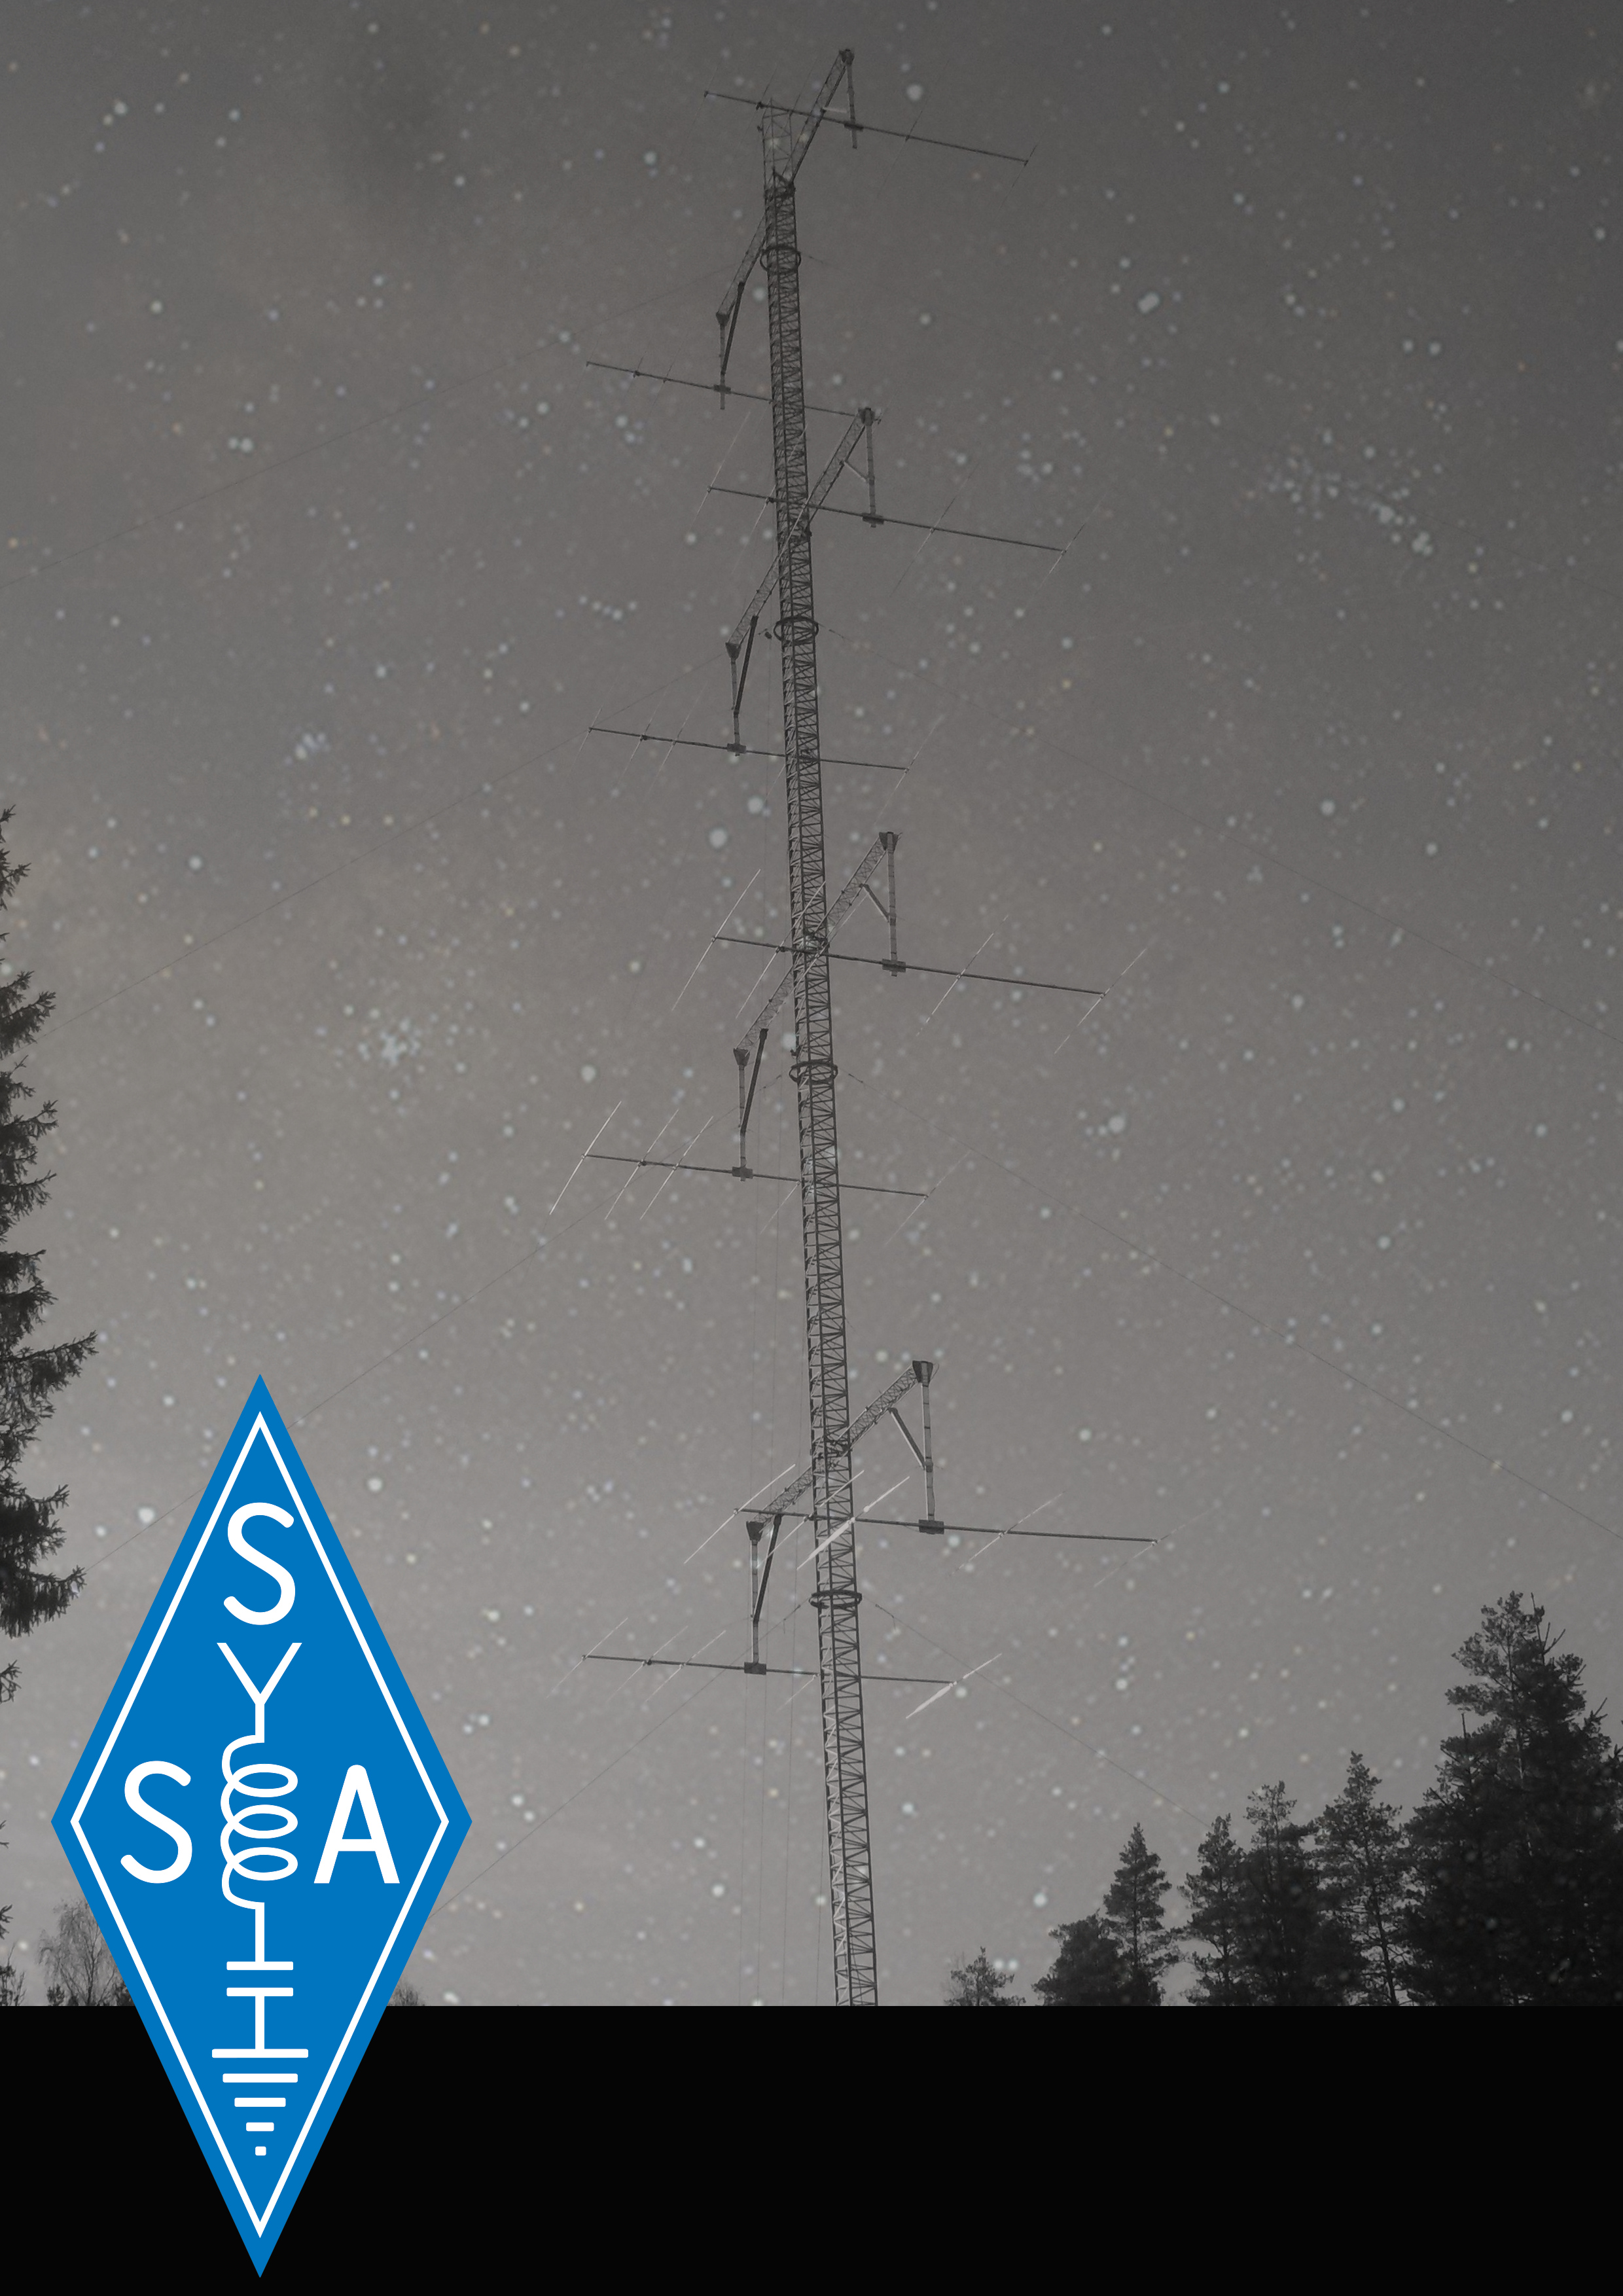
\includegraphics[width=\paperwidth,height=\paperheight,%
keepaspectratio]{images/koncept-front.jpg}%
\vfill
}}}


\newcommand\Backgroundtwo{%
\put(0,0){%
\parbox[b][\paperheight]{\paperwidth}{%
\vfill
\centering
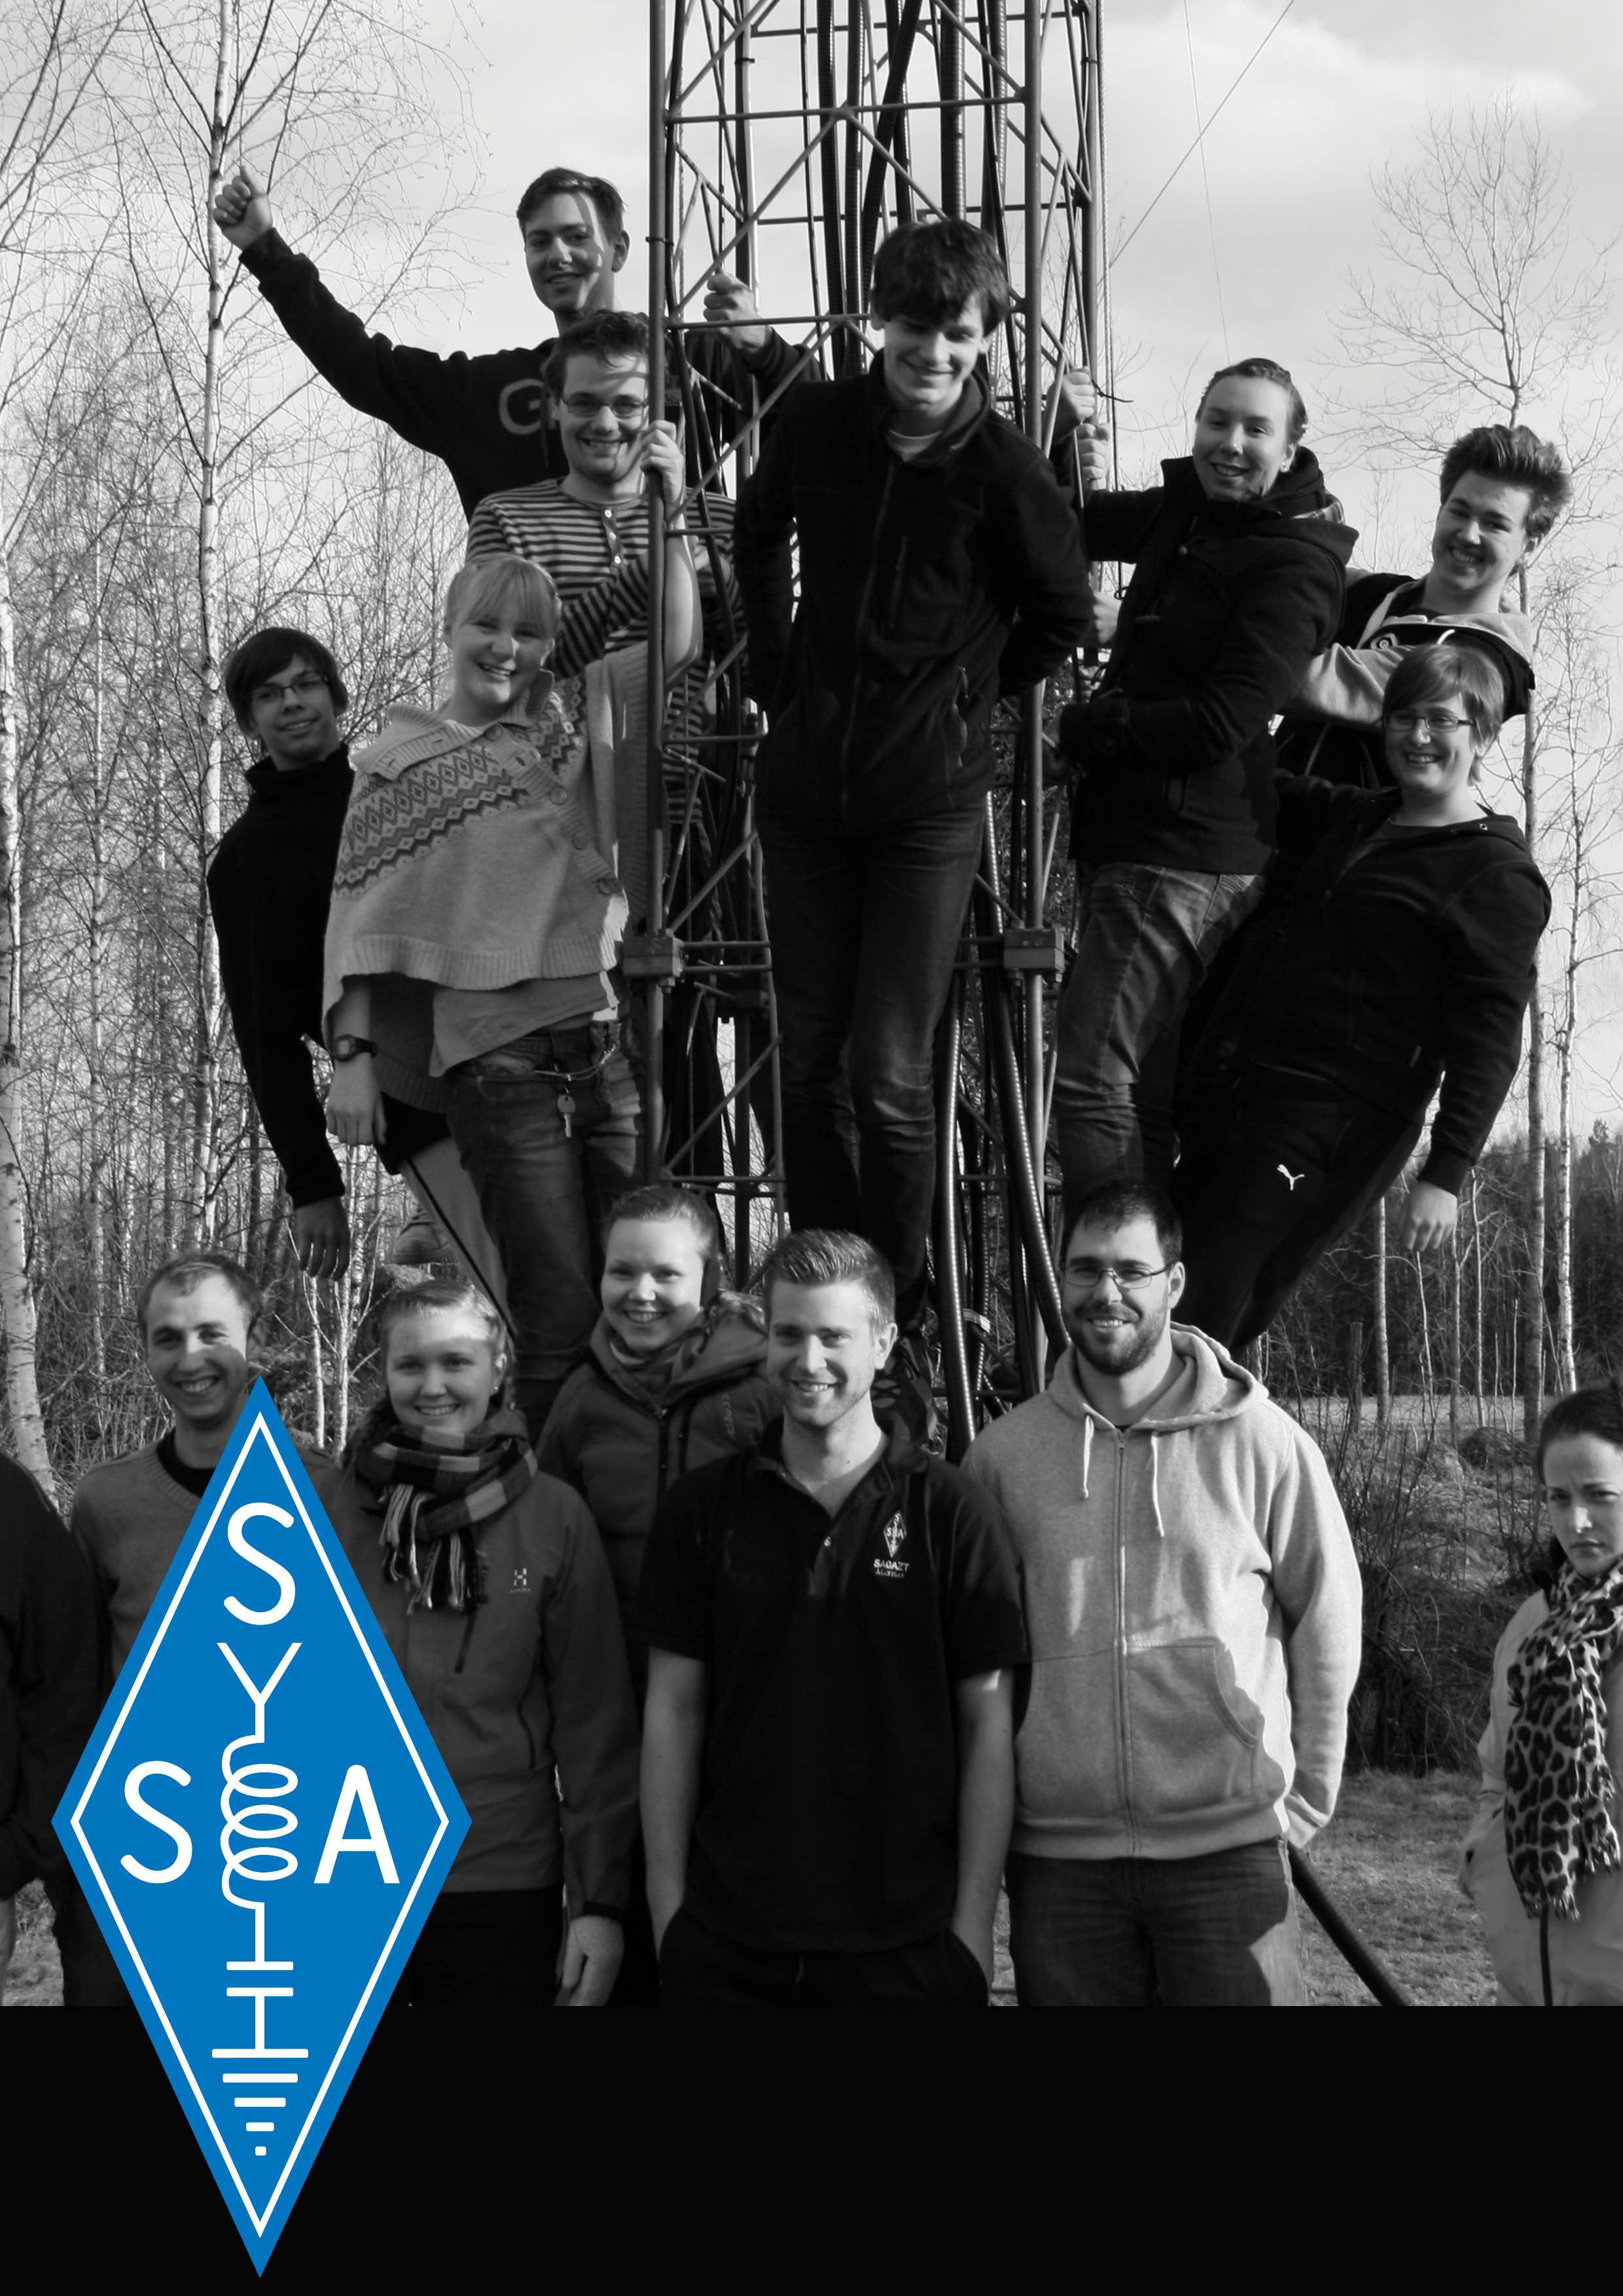
\includegraphics[width=\paperwidth,height=\paperheight,%
keepaspectratio]{images/koncept-larobok-front.jpg}%
\vfill
}}}



\newcommand\BackgroundPicLast{%
\put(0,0){%
\parbox[b][\paperheight]{\paperwidth}{%
\vfill
\centering

\includegraphics[width=\paperwidth,height=\paperheightsssss]{images/koncept-back.pdf}%
\vfill
}}}


\hyphenation{amatör-radio-certi-fikat kvarts-kristaller nät-an-slu-ten bär-vågs-am-pli-tud 
fas-änd-ring-en}
